\chapter{Lecture 9 - Power Series Solutions with MATLAB}
\label{ch:lec9}
\section{Objectives}
The objectives of this lecture are:
\begin{itemize}
\item Illustrate the solution of a linear IVP (with a 3-term recurrence) using Power Series.
\item Demonstrate \textbf\underline{a way} to analyze these solutions using MATLAB; and
\item demonstrate some expected elements of MATLAB style for this course.
\end{itemize}

\section{Solution of an IVP using Power Series}

Consider the following IVP:\marginnote{As before, we will assume $u = \sum\limits_{n=0}^{\infty}c_n x^n$.  This means that $u^{\prime} = \sum\limits_{n=1}^\infty n c_n x^{n-1}$, and $u^{\prime \prime} = \sum\limits_{n=2}^{\infty} n(n-1)c_nx^{n-2}$.}
\begin{align*}
\text{Governing Equation:   }& u^{\prime \prime}-(1+x)u = 0, \ \ u\in[0,5]\\
\text{Initial Conditions:   }& u(0) = 5, \ \ u^{\prime}(0) = 1
\end{align*}
Inserting our assumed power series solution into the governing equation gives us:
\begin{align*}
\sum\limits_{n=2}^{\infty}n(n-1)c_nx^{n-2} - (1+x)\sum\limits_{n=0}^{\infty}c_nx^n &= 0 \\
\sum\limits_{n=2}^{\infty}n(n-1)c_nx^{n-2} - \sum\limits_{n=0}^{\infty}c_nx^{n} - \sum\limits_{n=0}^{\infty}c_nx^{n+1} &= 0
\end{align*}
\marginnote[-1.0cm]{Note the effect of distributing $-(1-x)$ through the second summation.}
\noindent We need to evaluate the order of $x$ for the first term in each summation to determine if the summations are in phase:
\begin{equation*}
\underbrace{\sum\limits_{n=2}^{\infty}n(n-1)c_nx^{n-2}}_{x^0} - \underbrace{\sum\limits_{n=0}^{\infty}c_nx^{n}}_{x^0} - \underbrace{\sum\limits_{n=0}^{\infty}c_nx^{n+1}}_{x^1} = 0
\end{equation*}
To get the three summations in phase we need to strip off the first terms in the first and second summations so that all three summations start at $x^{1}$.  This gives us:
\begin{equation*}
2c_2 + \sum\limits_{n=3}^{\infty}n(n-1)c_nx^{n-2} - c_0 - \sum\limits_{n=1}^{\infty} c_nx^n -\sum\limits_{n=0}^{\infty}c_nx^{n+1} = 0
\end{equation*}

\begin{equation*}
2c_2 - c_0 + \underbrace{\sum\limits_{n=3}^{\infty}n(n-1)c_nx^{n-2}}_{\substack{k=n-2 \\ n=k+2}} - \underbrace{\sum\limits_{n=1}^{\infty} c_nx^n}_{\substack{k=n \\ n=k}} -\underbrace{\sum\limits_{n=0}^{\infty}c_nx^{n+1}}_{\substack{k=n+1 \\ n=k-1}} = 0
\end{equation*}
Substituting within each summation and combining terms gives us:
\begin{equation*}
(2c_2-c_0)x^0 + \sum\limits_{k=1}^{\infty}\left[(k+2)(k+1)c_{k+2} - c_k - c_{k-1} \right]x^k = 0
\end{equation*}
As usual, in order to satisfy this equation, the coefficients for each power of $x$ must be equal to zero.  For $x^0$ this means $2c_2 - c_0 = 0$;  For all the other powers of $x$, a \emph{three-term recurrence} involving $c_{k-1}$, $c_k$, and $c_{k+2}$ must be satisfied:
\begin{equation*}
c_{k+2} = \frac{c_k + c_{k-1}}{(k+2)(k+1)}
\end{equation*}
To help manage the complexity we will adopt the following strategy: \index{power series, three-term recurrance}
\begin{itemize}
\item Case 1: Arbitrarily set $c_0 \ne 0$, set $c_1 = 0$ and derive a solution.
\item Case 2: Arbitrarily set $c_0 = 0$, set $c_1 \ne 0$ and derive a second solution.
\end{itemize}
\marginnote[-1.75cm]{These two solutions will be linearly independent since the first will not have a linear term (proportional to $x$) and the second equation will not have a constant term (proportional to $1$).}

\vspace{0.5cm}

\noindent\textbf{Case 1: $c_0 \ne 0, \ \ c_1=0$}

\noindent Since $c_0 \ne 0$, we get $c_2 = \frac{c_0}{2}$. The coefficients derived for the first few values of $k$ are shown in the table to the right.
\begin{margintable}
\begin{tabular}{l|l}
\multicolumn{2}{l}{\textbf{Case 1:}} \\
$k=1$ & $k=2$ \\
$c_3 = \frac{c_0 + \cancelto{0}{c_1}}{(2)(3)} = \frac{c_0}{6}$ & $c_4 = \frac{\cancelto{0}{c_1}+c_2}{(3)(4)} = \frac{c_2/2}{12} = \frac{c_0}{24}$\\\hline
\multicolumn{2}{l}{$k=3$} \\
\multicolumn{2}{l}{$c_5 = \frac{c_2 + c_3}{(4)(5)} = \frac{c_0/2 + c_0/6}{20} = \frac{c_0}{30}$} \\
\end{tabular}
\end{margintable}
\noindent The solution we thus derive is shown below:
\begin{align*}
u_1 &= c_0 + c_1x + c_2x^2 + c_3x^3 + c_4x^4 + c_5x^5 + \cdots \\
u_1 &= c_0\left(1 + \frac{\cancelto{0}{c_1}}{c_0}x + \frac{c_2}{c_0}x^2 + \frac{c_3}{c_0}x^3 + \frac{c_4}{c_0}x^4 + \frac{c_5}{c_0}x^5 + \cdots \right) \\
u_1 &= c_0\left(1 + \frac{1}{2}x^2 + \frac{1}{6}x^3 + \frac{1}{24}x^4 + \frac{1}{30}x^5 + \cdots \right)
\end{align*}

\vspace{1.0cm}

\noindent\textbf{Case 2: $c_0 = 0, \ \ c_1 \ne 0$}

\noindent Since $c_1 = 0$ and $c_2 = \frac{c_0}{2}$, $c_2 = 0$.  The coefficients derived for the first few values of $k$ are shown in the table.
\begin{margintable}
\begin{tabular}{l | l}
\multicolumn{2}{l}{\textbf{Case 2:}} \\
$k=1$ & $k=2$ \\
$c_3 = \frac{\cancelto{0}{c_0}+c_1}{(2)(3)} = \frac{c_1}{6}$ & $c_4 = \frac{c_1 + \cancelto{0}{c_2}}{(3)(4)} = \frac{c_1}{12}$\\\hline
\multicolumn{2}{l}{$k=3$} \\
\multicolumn{2}{l}{$c_5 = \frac{\cancelto{0}{c_2}+c_3}{(4)(5)} = \frac{c_1/6}{20} = \frac{c_1}{120}$}\\
\end{tabular}
\end{margintable}
\noindent The solution we thus derive is shown below:
\begin{align*}
u_2 &= \cancelto{0}{c_0} + c_1x + c_2x^2 + c_3x^3 + c_4x^4 + c_5x^5 + \cdots \\
u_2 &= c_1 \left(x + \frac{\cancelto{0}{c_2}}{c_1}x^2 + \frac{c_3}{c_1}x^3 + \frac{c_4}{c_1}x^4 + \frac{c_5}{c_1}x^5 \cdots \right) \\
u_2 &= c_1 \left(x+\frac{1}{6}x^3 + \frac{1}{12}x^4 + \frac{1}{120}x^5 + \cdots \right)
\end{align*}
We now have two linearly independent solutions to the governing equation:
\begin{multline*}
u(x) = u_1(x) + u_2(x) = c_0\left(1 + \frac{1}{2}x^2 + \frac{1}{6}x^3 + \frac{1}{24}x^4 + \frac{1}{30}x^5 + \cdots \right) + \\ 
c_1\left(x + \frac{1}{6}x^3 + \frac{1}{12}x^4 + \frac{1}{120}x^5 + \cdots \right)
\end{multline*}
We are now ready to apply the initial conditions:  
\begin{align*}
u(0) &= c_0 = 5 \\
u^{\prime}(0) &= c_1 = 1
\end{align*}
So the final solution is:
\begin{multline*}
u(x)= 5\left(1 + \frac{1}{2}x^2 + \frac{1}{6}x^3 + \frac{1}{24}x^4 + \frac{1}{30}x^5 + \cdots \right) + \\ 
\left(x + \frac{1}{6}x^3 + \frac{1}{12}x^4 + \frac{1}{120}x^5 + \cdots \right)
\end{multline*}

\section{Generating and Plotting Solutions with MATLAB}
The point of doing all of this math is to gain insight.  In many cases systems of interest are subject to physical laws that are expressed in the form of differential equations; we solve these differential equations to better understand how the systems will perform.  

\newthought{There are two problems} that I hope to address with this section:  
\begin{enumerate}
\item It is both tedious and error-prone to generate the coefficients for the series solution.  We worked hard to construct a small portion of the power series solutions and we hope that we did it without any errors.  With a modest amount of programming effort, we will construct a script that can build a series solution with as many terms as we would like.  With conscientious debugging we can be sure that, floating point round-off errors aside, the calculations are done quickly and correctly.  

\item We may gain considerably more insight from the solution if we can create a plot.  If the plot can easily be made with the same computing tools used to generate the solution, we can get this insight with very little extra work.
\end{enumerate}

We will use MATLAB to generate and plot the solutions.  We start our MATLAB script in the same way we will start \emph{all} of our MATLAB scripts, with the following three lines:\marginnote{This is done in accordance with the MATLAB Style Rule \#1.  The MATLAB Style Rules are listed in the Appendices and I will try to exemplify the rules in the code I provide as examples in the lectures.}
\begin{lstlisting}[name=lec9_ex1,style=myMatlab]
clear
clc
close 'all'
\end{lstlisting}
Next we will specify the number of terms that we will retain from the infinite series and allocate arrays in which the coefficients will be stored.\marginnote{We will use two arrays to store the coefficients; one for $u_1(x)$ and the other for $u_2(x)$.  Pre-allocation in this way is done in accordance with MATLAB Style Rule \# 7, and the comments are in accordance with Rule \# 2. Use of short but meaningful variable names is prescribed in Rule \#3.}
\begin{lstlisting}[name=lec9_ex1,style=myMatlab]
n=25;
C1 = nan(1,n); % coefficients for u1(x)
C2 = nan(1,n); % coefficients for u2(x)
\end{lstlisting}
Recall that for $u_1(x)$ we applied our strategy for ``case 1'' in which we assumed that $c_0 \ne 0$ and $c_1 = 0$.  This implied that $c_2 = c_1/2$ while the recurrence relation was used for all of the other coefficients.  When we applied the initial conditions we found that $c_0=5$ for $u_1(x)$.  The code snippet below accomplishes these tasks.\marginnote{Note how each line of MATLAB in this listing is terminated with a semicolon.  This is to suppress the output to the command line that would otherwise happen each time we make an assignment to a variable.  While this output might be helpful during debugging, during any other time it is distracting (drowning out other, more useful output) and slows code execution.  The extensive, non-readable output that would result from omitting the semicolons is indicative of a violation of MATLAB Style Rule \#4.}
\begin{lstlisting}[name=lec9_ex1,style=myMatlab]
C1_0 = 5; % c_0 for u1(x), handled separatly since MATLAB array 
% indices start at 1
C1(1) = 0; % c_1 for u1(x)
C1(2) = C1_0/2; % c_2 for u1(x)

% handle the k=1 case separately since it involves the term C1_0
k = 1;
C1(k+2) = (C1(k) + C1_0)/((k+1)*(k+2));

for k=2:(n-2)
  C1(k+2) = (C1(k) + C1(k-1))/((k+1)*(k+2));
end
\end{lstlisting} 
Now we have calculated all of the desired coefficients, we are ready to construct the first solution.\marginnote{Here $u_1(x)$ is created as an \emph{anonymous} function.  We begin with the constant term on line 28 and build up the function term-by-term within the \emph{for} loop on line 30. The indentation you see in these code blocks has been done automatically by the ``smart indentation'' feature of MATLAB's built-in editor.  This is retained in accordance with MATLAB Style Rule \#6.}
\begin{lstlisting}[name=lec9_ex1,style=myMatlab]
u1 = @(x) C1_0;
for k = 1:n
  u1 = @(x) u1(x) + C1(k)*x.^k;
end
\end{lstlisting}
We continue in this same vein to construct $u_2(x)$ as we did in our ``case 2'' strategy and construct the solution $u(x) = u_1(x) + u_2(x)$.
\begin{lstlisting}[name=lec9_ex1,style=myMatlab]
C2_0 = 0; % c_0 for u2(x)
C2(1) = 1; % from the initial condition
C2(2) = C2_0/2; % just adding for consistency's sake

k=1;
C2(k+2) = (C2(k) + C2_0)/((k+1)*(k+2));
for k = 2:(n-2)
  C2(k+2) = (C2(k) + C2(k-1))/((k+1)*(k+2));
end

u2 = @(x) C2_0;
for k = 1:n
  u2 = @(x) u2(x) + C2(k)*x.^k;
end

u = @(x) u1(x) + u2(x);
\end{lstlisting}

\vspace{2.0cm}

\newthought{Now that we} have a MATLAB representation of the solution, let us create a plot.  One way to make such a plot is shown in the listing below; the output is shown in Figure \ref{fig:lec9_fig1}.:
\begin{marginfigure}
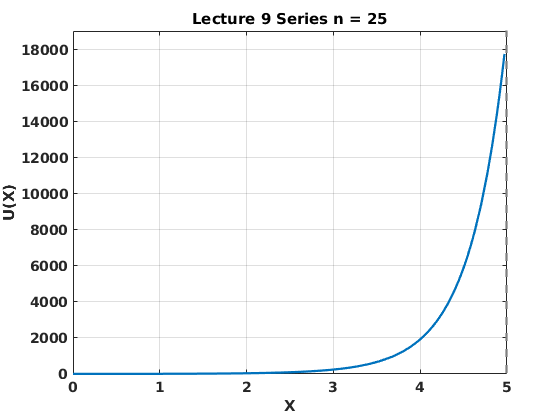
\includegraphics{lec9_fig1.png}
\caption{Power series solution to $u^{\prime \prime}-(1+x)u=0, \ u(0)=5,\ u^{\prime}(0)=1$.}
\label{fig:lec9_fig1}
\end{marginfigure}
\begin{lstlisting}[name=lec9_ex1,style=myMatlab]
xMin = 0; xMax = 5;
figure(1)
fplot(u,[xMin, xMax],'linewidth',2);
title_str = sprintf('Lecture 9 Series n = %d',n);
title(title_str,'fontsize',18,'fontweight','bold');
xlabel('X','fontsize',16,'fontweight','bold');
ylabel('U(X)','fontsize',16,'fontweight','bold');
set(gca,'fontsize',12,'fontweight','bold');
grid on
\end{lstlisting}
\marginnote{\textbf{Note:} Pay particular attention to the formatting details of the plot.  There is a title along with axis-labels for both the x- and y-axis; fonts are bold and sized in a systematic way.  Grid lines are also used to make the graph more readable.  These details have all been added in observance of MATLAB Style Rule \#4. 

The variables \lstinline[style=myMatlab]{xMin} and \lstinline[style=myMatlab]{xMax} on line 39 has been included in accordance with Rule \#8.  The fact that both variables are initialized on the same line is a common exception to Rule \#9.}
\newthought{A few more} details are worth noting.  
\begin{enumerate}
\item We know our solution is inexact since we truncated the infinite power series and used finite-precision arithmetic while calculating the coefficients for those terms we \emph{did} bother to include.  Still, we might want to know \emph{how wrong} the solution is.
\item Taking a more positive tack, we might ask how much \emph{better} the solution gets when we add more terms to our solution.
\end{enumerate}
To answer either of these questions, we will need access to the solution of the IVP.  For this lecture, we will take a numeric solution generated using MATLAB's built-in IVP-solving tool \emph{ODE45} as ``the solution.''\marginnote[-1.0cm]{Use of tools such as \emph{ODE45} will be treated in the numerical methods section.}
\begin{marginfigure}
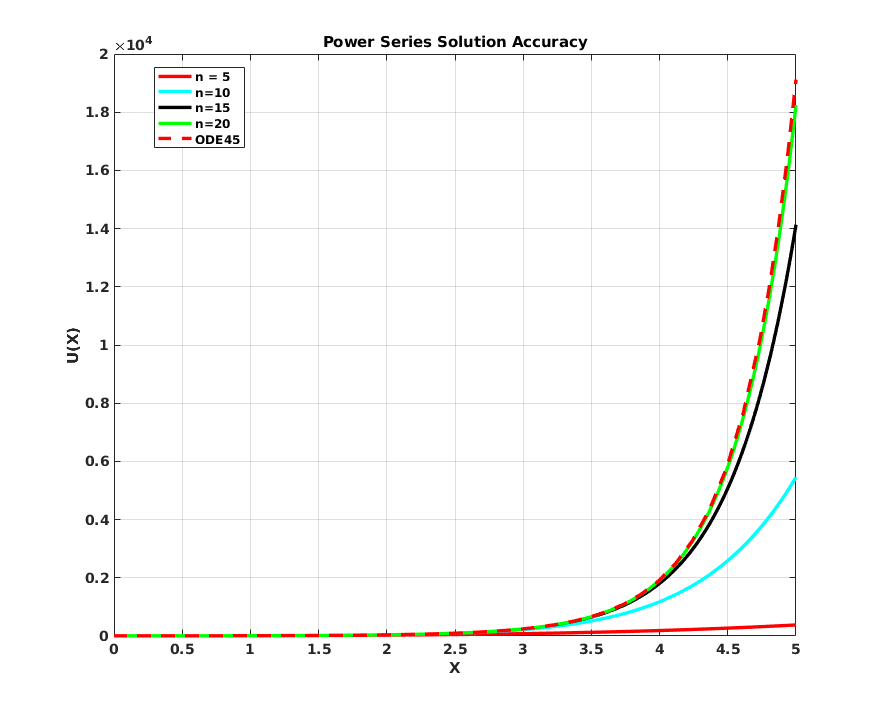
\includegraphics{lec9_ps_compare.png}
\caption{Power series solution with different values of $n$.}
\label{fig:lec9_ps_compare}
\end{marginfigure}

Power series results for various values of $n$ are compared to the numerical solution in Figure \ref{fig:lec9_ps_compare}.  Some things to notice:
\begin{enumerate}
\item The solution gets worse the further one gets from zero; and
\item The solution gets better for larger values of $n$.  
\end{enumerate}
Neither of these observations should be particularly surprising but there is value to seeing it in your results. It adds confidence to the proposition that your (approximate) solution is correct.

\newthought{As a last note} it should be pointed out that, while plots like that shown in Figure \ref{fig:lec9_ps_compare} gives a good qualitative feel for how the solution is improving as the number of power series terms increases, a quantitative measure for correctness is preferable.  In Figure \ref{fig:lec9_ps_converge} a quantitative measure---the relative error in the 2-norm---is used to quantify the difference between different power series solutions and the solution generated using \emph{ODE45}.  Details of this error measure will be discussed in future lectures.
\begin{marginfigure}
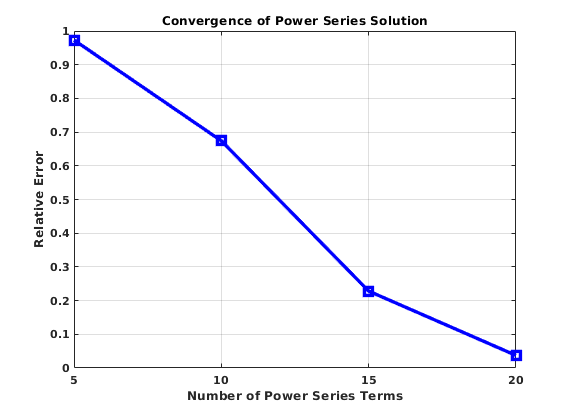
\includegraphics{lec9_ps_converge.png}
\caption{Convergence of the power series solution to the numeric solution.}
\label{fig:lec9_ps_converge}
\end{marginfigure}   

